\section{Results}
\label{sec:results}

Following the implementation details presented in the previous section
we created a tool that automatically, given a dump of a Tor/Firefox
tab, will find the DocumentElement. Afterwards, it will extract the
DOM nodes while checking their type. For the text and comment nodes,
the tool will read the \textit{mText} field while for "a", "img" and
"video" nodes it reads the corresponding source fields described in
the previous section. The output of the tool consists of: URL of the
current tab, referrer of the current tab and the incomplete
reconstructed HTML which is put in the "./dump.html" file. The created
HTML has the same text nodes but the structure of the tree often is
different. This happens because there are nodes in the DOM that are
not shown in the browser inspector. These nodes are not part of the
HTML, they are added by the browser for various reasons that we do not
fully know. In this section, we show how we run the tool and what
output we get for 3 websites: os3.nl\cite{os3nl}, ccf website (clicked
on the CCF link)\cite{os3ccfnl} and
http://zqktlwi4fecvo6ri.onion/wiki/index.php/Main\_Page which is the
full version of the hidden wiki\cite{thehiddenwiki}.

\subsection{Usage}
The tool is written in Python and takes as parameter the directory
containing the dumped Tor virtual address space. A directory is needed
due to the way that Volatility extracts the address space: each
virtual mapping is put in a separate file. This dump is extracted in
advance using Volatility's \textbf{linux\_dump\_map (dump\_map for
  windows)} command.

\subsection{Simple Website}
As a simple test, we typed \textbf{os3.nl} in the URL bar and hit
enter. When we run the tool, we get the output in
figure~\ref{img:output1}. We can see the correct URL return and the
null referrer field (since the URL was typed).

\begin{figure}[h]
  \centering 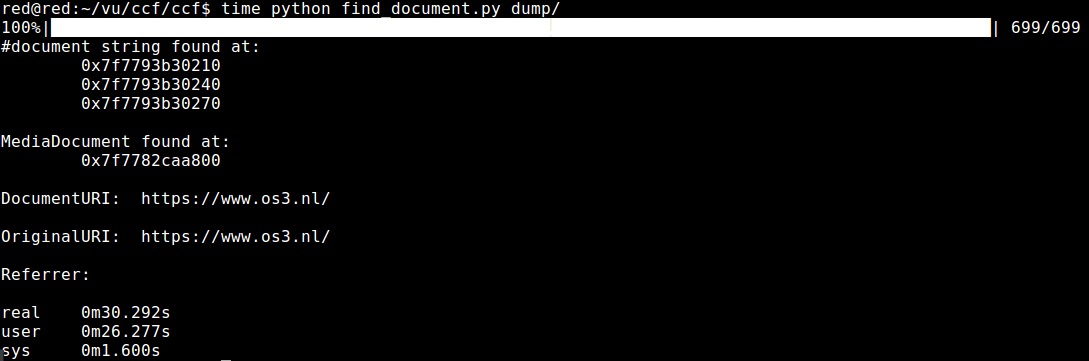
\includegraphics[scale=0.35]{output1}
  \caption{Output when running the tool on the dump generated for the
    os3.nl visit.}
  \label{img:output1}
\end{figure}

When we look at the HTML produced, we can see that the text is the
same but the lack of styling and attributes makes the pages look very
different. A small comparison can be seen in
figure~\ref{fig:os3_compare}. This HTML mismatch is expected and can
be improved with future work on attributes and CSS styles. However,
content can arguably be deduced during an investigation, even from
incomplete recreated HTML.

\begin{figure}[h]
  \begin{subfigure}{\linewidth} \centering
    
\includegraphics[scale=0.35]{os3_orig1}
    \caption{Original os3.nl website.}
  \end{subfigure}\\[1ex]

  \begin{subfigure}{\linewidth} \centering
    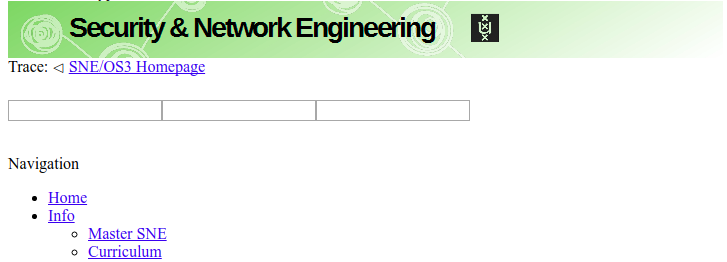
\includegraphics[scale=0.35]{os3_recovered1}
    \caption{Reconstructed HTML from os3.nl website.}
  \end{subfigure}
  \caption{Comparison between original and reconstructed os3.nl HTML.}
  \label{fig:os3_compare}
\end{figure}

\subsection{Referrer}
In order to check the referrer field, we clicked on the "CCF" link of
the previously browsed website. The result, as seen in
figure~\ref{img:output2} is correct: the referrer points to the os3.nl
website where we clicked the link. The recovered HTML again contains
true text but completely wrong styling, although some elements, such
as tables, maintain a good aspect even without styling as seen in
figure~\ref{fig:ccf_compare}.

\begin{figure}[h] \centering 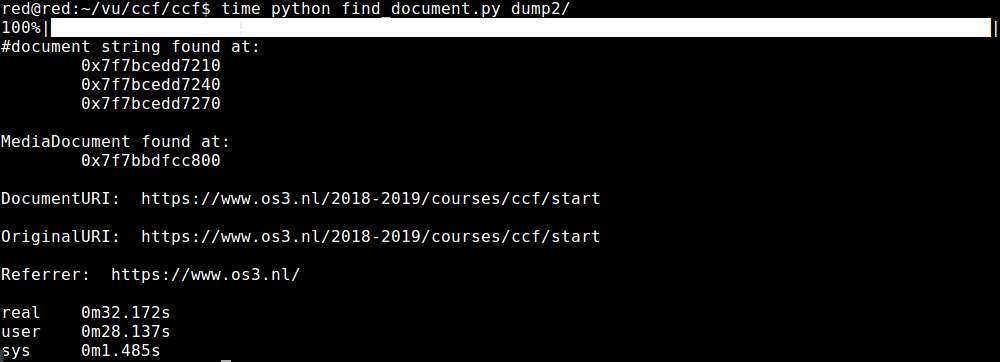
\includegraphics[scale=0.35]{output2}
  \caption{Output when running the tool on the dump generated for the
    CCF link click.}
  \label{img:output2}
\end{figure}

\begin{figure}[h]
  \begin{subfigure}{\linewidth} \centering
    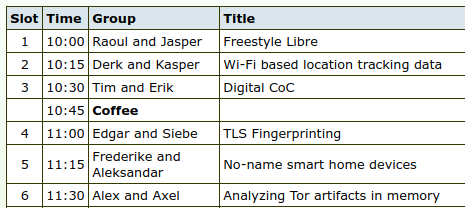
\includegraphics[scale=0.35]{ccf_orig1}
    \caption{Original ccf website.}
  \end{subfigure}\\[1ex]

  \begin{subfigure}{\linewidth} \centering
    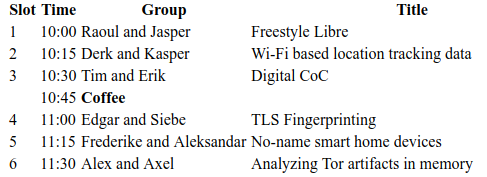
\includegraphics[scale=0.35]{ccf_recovered}
    \caption{Reconstructed HTML from ccf website.}
  \end{subfigure}
  \caption{Comparison between original and reconstructed ccf HTML.}
  \label{fig:ccf_compare}
\end{figure}

\subsection{Onion Website}
We also tried the tool on a \textit{.onion} website. Our expectation
was that the tool will work the same since the same exact memory
structures are used to represent the DOMs for \textit{.onion}
websites. As can be seen in figures~\ref{img:output3}
and~\ref{fig:hidden_compare} the results are similar to normal
webpages. An important observation is that for \textit{.onion}
websites, opening the reconstructed HTML with a default browser will
not show any images due to their origin being behind a \textit{.onion}
URL. The tool still recovers the correct source as can be seen
in~\ref{img:onion_img}.

\begin{figure}[h]
  \centering 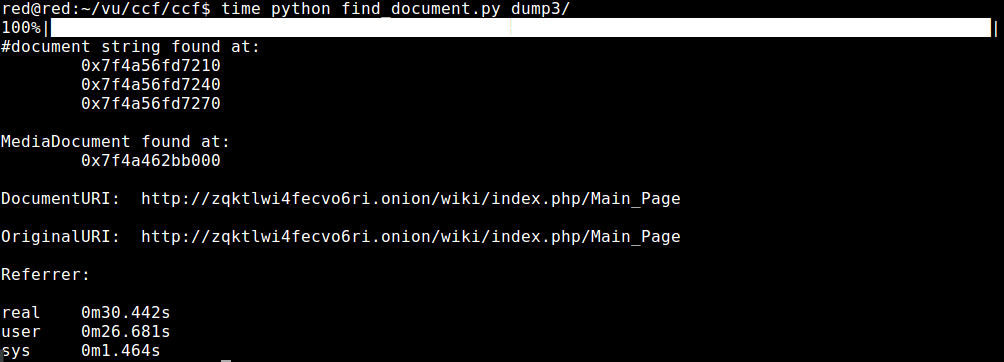
\includegraphics[scale=0.35]{output3}
  \caption{Output when running the tool on the dump generated for the
    hidden wiki \textit{.onion} website.}
  \label{img:output3}
\end{figure}

\begin{figure}[H]
  \begin{subfigure}{\linewidth}
    \centering 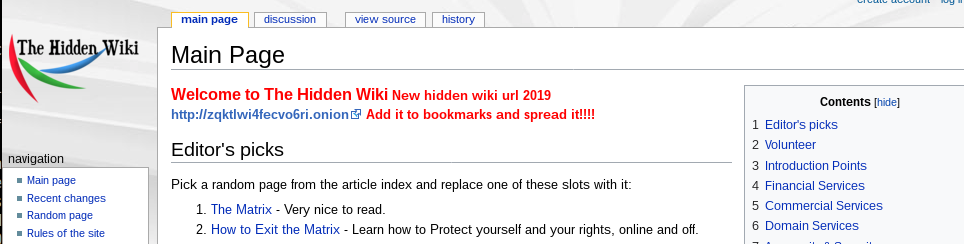
\includegraphics[scale=0.35]{hidden_orig}
    \caption{Original hidden wiki website.}
  \end{subfigure}\\[1ex]

  \begin{subfigure}{\linewidth}
    \centering 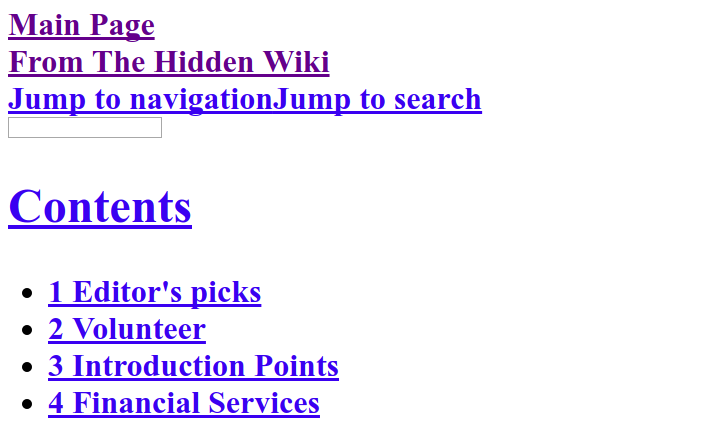
\includegraphics[scale=0.35]{hidden_recovered}
    \caption{Reconstructed HTML from hidden wiki website.}
  \end{subfigure}
  \caption{Comparison between original and reconstructed hidden wiki
    HTML.}
  \label{fig:hidden_compare}
\end{figure}

\begin{figure}[H]
  \centering 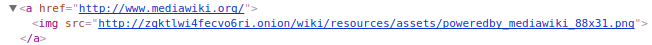
\includegraphics[scale=0.65]{onion_img}
  \caption{img element reconstructed with correct src.}
  \label{img:onion_img}
\end{figure}

\subsection{Run time}
In all of the test cases we run the tool under the unix \textbf{time}
command to see the exact durations of the execution. We show that for
dumps of 1.7GB the tool take approximately 30 seconds to recover the
data, where the biggest part is spent finding the
DocumentElement. This demonstrates that the approach is quite fast and
can parse through big HTML documents in matters of minutes.
